Using a learning rate of 0.0001, and having implemented all of the
improvements mentioned in \cref{ch:environment}, we trained a \gls{ppo} agent
for 60 million steps. The results can be seen in \cref{fig:ppo}.

\begin{figure}[H]
    \begin{subfigure}{0.45\textwidth}
        \centering
        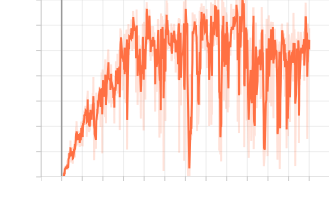
\includegraphics[width=\textwidth]{img/ppo_len_mean.png}
        \caption{Mean episode length}
        \label{fig:ppo_len_mean}
    \end{subfigure}
    \begin{subfigure}{0.45\textwidth}
        \centering
        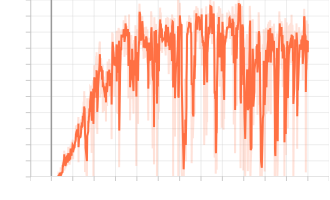
\includegraphics[width=\textwidth]{img/ppo_rew_mean.png}
        \caption{Mean episode reward}
        \label{fig:ppo_reward_mean}
    \end{subfigure}
    \caption{PPO training results}
    \label{fig:ppo}
\end{figure}

As we can see in \cref{fig:ppo}, the agent is able to learn to play the game
quite well, with the mean episode length and the mean episode reward increasing
steadily throughout the first 20 million steps. However, after 20 million steps,
the mean episode length and the mean episode reward start to fluctaute,
although this does not seem to affect the overall performance of the agent.

Through testing, the agent is able to complete several levels of the game,
which is a significant improvement over the previous results. The agent is
also able to complete the game somewhat consistently, although it still has
a tendency to jump off the platform and die (but less than with \gls{ddqn}).
This could be due to some of the parameters of the algorithm not being
optimized, or it could be due to the factors surrounding the number of lives
mentioned in \cref{ch:environment}.

However, further investigation into the underlying working of the algorithm
is needed to determine the exact cause of the issue. This could involve
looking at the gradients of the policy and the value function, or it could
involve looking at the advantage function and how it is computed.